% =============================================================================
% Progress Report (5-page version) — Context-Conditioned Sequential Keypoint
% Density Estimation
% Doruk Topcu (N25142281), Hacettepe University
% Template: ICLR 2025 Conference Submission
% =============================================================================
\documentclass{article}
\usepackage{iclr2025_conference,times}

\usepackage{amsmath,amssymb,amsthm}
\usepackage{graphicx}
\usepackage{booktabs}
\usepackage{hyperref}
\usepackage{url}
\usepackage{xcolor}
\usepackage{tikz}
\usetikzlibrary{decorations.pathreplacing,positioning}

\title{Context-Conditioned Sequential Keypoint Density Estimation\\
       for Traffic Hazard Detection \\ \vspace{0.4em}
       {\large Progress Report}}

\author{Doruk Topcu \\
        Department of Computer Engineering \\
        Hacettepe University \\
        \texttt{doruktopcu@hacettepe.edu.tr} \\
        \texttt{N25142281}}

\iclrfinalcopy

\begin{document}
\maketitle

\begin{abstract}
The Sequential Keypoint Density Estimator (SeeKer / SKDE) is a recent
ICCV~2025 baseline for skeleton-based video anomaly detection that factorizes
the joint density of a pedestrian's 2D keypoint trajectory autoregressively.
SeeKer is \emph{environmentally blind}: each skeleton is modelled in
isolation from the surrounding scene, which is fundamentally limiting in
traffic-hazard scenarios where the danger lies in pedestrian--object
interactions. We propose \textbf{CCSKDE}, a minimal extension that injects a
per-frame environmental context vector $C_t$ --- derived offline from
YOLOv11 detections of non-pedestrian scene elements --- into SeeKer's
autoregressive backbone via an unconditional MADE shortcut, preserving
keypoint causality. On ShanghaiTech, CCSKDE matches the reproduced SeeKer
peak ($0.78$ AUROC) while improving training stability ($+1.9$~pp mean
AUROC). A spatiotemporally shuffled-$C_t$ ablation, with identical parameter
count, lags the aligned model by $2.4$~pp, confirming that context
provides genuine signal beyond extra capacity.
\end{abstract}

% -----------------------------------------------------------------------------
\section{Problem Definition}
\label{sec:problem}

Video anomaly detection (VAD) identifies frames or events whose appearance,
motion, or interaction patterns deviate from those observed in a training
set of \emph{normal} videos. Modern VAD pipelines increasingly operate on
privacy-preserving 2D human skeletons rather than raw RGB pixels, yielding
lower-dimensional inputs that are invariant to lighting and appearance bias.
Within this family, the \emph{Sequential Keypoint Density Estimator}
(SeeKer) of \citet{delic2025seeker} is a particularly elegant baseline: it
treats a pedestrian's pose trajectory as a high-dimensional time series and
estimates its joint density via a keypoint-level autoregressive
factorization, where each 2D keypoint is predicted as a Gaussian conditioned
on previously generated keypoints in the same and earlier frames. Despite
using only a small masked fully-connected (MADE)
network~\citep{germain2015made}, SeeKer matches or exceeds heavier flow- and
graph-based competitors on standard
benchmarks~\citep{hirschorn2023normalizing,liu2018future}.

\paragraph{Limitation we address.}
SeeKer's distribution is conditioned only on the pedestrian's own past
keypoints; it never observes \emph{what else is in the scene}. A pedestrian
walking at constant velocity in a calm campus square and the same pedestrian
walking at the same velocity into the path of a moving vehicle yield
identical SeeKer likelihoods --- yet the latter is precisely the event we
need to flag. We extend SeeKer with a minimal, mathematically faithful
conditioning mechanism on a per-frame \emph{environmental context vector}
$C_t$, so that the predicted keypoint distribution can sharpen (smaller
covariance) when the pedestrian is in a high-risk spatial configuration.

\paragraph{Challenges.}
The problem is non-trivial for three reasons.
(i)~\textbf{Unsupervised conditioning}: VAD is one-class, so we must learn
which contextual configurations are normal without any hazard labels.
(ii)~\textbf{Preserving the autoregressive factorization}: naively
concatenating $C_t$ to MADE's input breaks the keypoint mask, so
conditioning must be injected as an unconditional shortcut while
keypoint-to-keypoint causality is left intact.
(iii)~\textbf{Generalization across scenes}: ShanghaiTech contains 13 camera
viewpoints, so $C_t$ must be a scene-scale-invariant function of
pedestrian--object geometry rather than absolute image coordinates.

% -----------------------------------------------------------------------------
\section{Related Work}
\label{sec:related}

\paragraph{Skeleton-based VAD.}
\citet{morais2019messagepassing} introduced one of the first skeleton-only
VAD pipelines using a recurrent message-passing network;
\citet{markovitz2020graph} cast normal motion as soft-clustering of
spatio-temporal graph embeddings. STG-NF~\citep{hirschorn2023normalizing}
fits a normalizing flow over spatio-temporal joint graphs and was the state
of the art on ShanghaiTech-HR until SeeKer. Our work builds directly on
SeeKer's masked-FC formulation.

\paragraph{Density estimation backbones.}
SeeKer's core is MADE~\citep{germain2015made}; related neural density
estimators (RealNVP~\citep{dinh2017realnvp}, Glow~\citep{kingma2018glow})
require multiple coupling layers but produce exact log-likelihoods.
SeeKer demonstrates that the simpler masked-FC formulation is sufficient
for VAD scoring and substantially cheaper.

\paragraph{Context-aware anomaly detection.}
A separate strand of VAD literature injects scene/object information into
the scorer. \citet{ionescu2019object} use per-object features and one-class
SVMs; \citet{georgescu2021background} use background-aware self-supervised
pretexts; HSC~\citep{sun2023hierarchical} and
SSMTL++~\citep{georgescu2022ssmtl} combine multiple object-level signals.
To our knowledge, no prior work injects an explicit
proximity-to-non-pedestrian context vector into an autoregressive keypoint
density estimator.

\paragraph{Object detection, dataset, pose extraction.}
We use YOLOv11~\citep{ultralytics2024yolov11} for offline detection of
non-pedestrian scene elements. ShanghaiTech
Campus~\citep{liu2018future} comprises 13 outdoor scenes, 437 videos, and a
mix of pedestrian/bicycle/vehicle activity --- the natural benchmark for
our hypothesis. We use AlphaPose COCO-17~\citep{fang2017rmpe} skeletons
(converted to COCO-18 with a synthetic neck, following SeeKer) released
with STG-NF for full reproducibility.

% -----------------------------------------------------------------------------
\section{Method}
\label{sec:method}

\subsection{Baseline: SeeKer}
\label{ssec:baseline}
Let a pedestrian track be a sequence of $T$ frames, each containing $V=18$
COCO-18 2D keypoints, denoted $X_{t,n} \in \mathbb{R}^{2}$. SeeKer
factorizes the joint density of the entire track as
\begin{equation}
\label{eq:seeker_factor}
p_{\theta}\!\left(X_{1:T}\right) \;=\;
\prod_{t=1}^{T} \prod_{n=1}^{V}
p_{\theta}\!\left(X_{t,n}\,\big|\, X_{t,<n},\, X_{<t}\right).
\end{equation}
Each conditional is a 2D Gaussian
$\mathcal{N}(\mu_{\theta}, \Sigma_{\theta})$ whose mean and Cholesky factor
of $\Sigma_{\theta}^{-1}$ are produced by a single masked fully-connected
network (\emph{MADEPartial}). The keypoint-level autoregressive constraint
is enforced by binary masks; SeeKer adapts the masking so conditioning is
causal both \emph{across} time and \emph{within} the keypoint ordering of
the current frame. Training minimizes the negative log-likelihood of
Eq.~\ref{eq:seeker_factor} on \emph{normal} sequences only. At inference,
each frame's score is the per-keypoint Mahalanobis-style NLL,
Gaussian-smoothed and optionally weighted by AlphaPose detection
confidence.

\subsection{Proposed extension: CCSKDE}
\label{ssec:ccskde}
We make the predicted distribution \emph{context-aware} by introducing a
per-frame context vector $C_t$:
\begin{equation}
\label{eq:ccskde_factor}
p_{\theta}\!\left(X_{t,n}\,\big|\, X_{t,<n},\, X_{<t},\, C_t\right).
\end{equation}

\paragraph{Constructing $C_t$.}
For each frame $t$ we run YOLOv11 on the raw RGB frame and retain
non-pedestrian classes that are plausible campus hazards: \texttt{car},
\texttt{truck}, \texttt{bus}, \texttt{motorcycle}, \texttt{bicycle}. For each
detection $b$ with bounding-box centre $(x_b, y_b)$, we compute the
diagonal-normalized image-space distance to the pedestrian's skeleton
centroid $\bar{x}_t$:
\(
d_{t,b} = \lVert (x_b, y_b) - \bar{x}_t \rVert_2 / \sqrt{H^2 + W^2}\,.
\)
We aggregate per class via inverse minimum distance and a count of objects
within a fixed radius:
\begin{equation}
C_t \;=\; \big[\,1/d^{\min}_{c_1},\,n^{\le r}_{c_1},\,
                 1/d^{\min}_{c_2},\,n^{\le r}_{c_2},\,\dots\,\big]
\;\in\;\mathbb{R}^{2K},
\end{equation}
with $K=5$ hazard classes and $r=0.15$. Frames with no relevant detection
get a zero vector. The design is fixed-dimension regardless of object
count, monotonic in proximity, and computed once offline.

\paragraph{Injection into the autoregressive backbone.}
We treat $C_t$ as an \emph{unconditional shortcut input}: its entries are
appended to the input vector and assigned a constant ``zero-degree'' label
in MADE's connectivity scheme. Concretely, only the input-layer mask is
altered (the columns corresponding to $C_t$ are set to all-ones); no
parameter is removed and no other mask changes. This guarantees every
output neuron may attend to every entry of $C_t$, while
keypoint-to-keypoint causality is exactly preserved
(see Fig.~\ref{fig:made_mask}). We verified the latter empirically with a
Jacobian test: across the current-frame keypoint output block, every $C_t$
entry reaches every output
($\partial \mu_i / \partial C_{t,j} \neq 0$ for all $j$), and zero
forbidden keypoint-to-keypoint paths leak.

\begin{figure}[t]
\centering
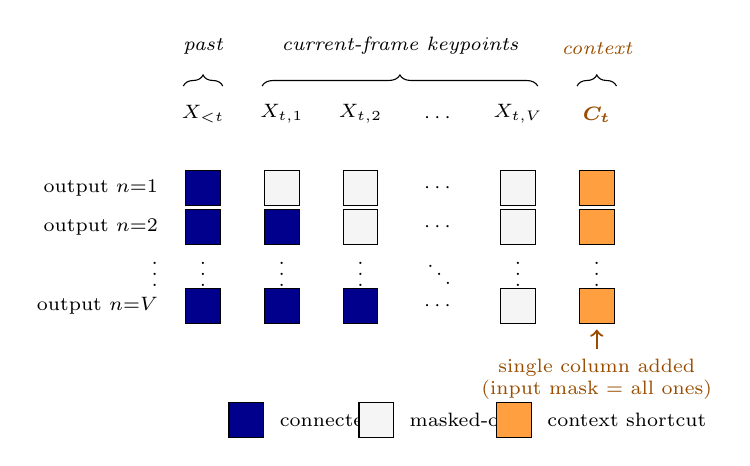
\begin{tikzpicture}[
    on/.style ={draw, fill=blue!55!black, minimum size=4.4mm, inner sep=0pt},
    off/.style={draw, fill=gray!8,        minimum size=4.4mm, inner sep=0pt},
    ctx/.style={draw, fill=orange!75,     minimum size=4.4mm, inner sep=0pt},
    rowlbl/.style={font=\scriptsize, anchor=east},
    collbl/.style={font=\scriptsize, anchor=south},
    grouplbl/.style={font=\scriptsize\itshape, anchor=south}
]
% Column header labels (input symbols)
\node[collbl] at (0, 2.20) {$X_{<t}$};
\node[collbl] at (1, 2.20) {$X_{t,1}$};
\node[collbl] at (2, 2.20) {$X_{t,2}$};
\node[collbl] at (3, 2.20) {$\cdots$};
\node[collbl] at (4, 2.20) {$X_{t,V}$};
\node[collbl, text=orange!60!black] at (5, 2.20) {$\boldsymbol{C_t}$};

% Group brackets
\draw[decorate, decoration={brace, raise=14pt, amplitude=4pt}]
     (-0.25, 2.30) -- (0.25, 2.30)
     node[grouplbl, midway, yshift=22pt] {past};
\draw[decorate, decoration={brace, raise=14pt, amplitude=4pt}]
     (0.75, 2.30) -- (4.25, 2.30)
     node[grouplbl, midway, yshift=22pt] {current-frame keypoints};
\draw[decorate, decoration={brace, raise=14pt, amplitude=4pt}]
     (4.75, 2.30) -- (5.25, 2.30)
     node[grouplbl, midway, yshift=22pt, text=orange!60!black] {context};

% Row 1: output for n=1 -- past on, all current keypoints off, C_t on
\node[on]  at (0, 1.5) {}; \node[off] at (1, 1.5) {};
\node[off] at (2, 1.5) {}; \node[font=\scriptsize] at (3, 1.5) {$\cdots$};
\node[off] at (4, 1.5) {}; \node[ctx] at (5, 1.5) {};
\node[rowlbl] at (-0.45, 1.5) {output $n{=}1$};

% Row 2: n=2 -- past on, X_{t,1} on, rest off, C_t on
\node[on]  at (0, 1.0) {}; \node[on]  at (1, 1.0) {};
\node[off] at (2, 1.0) {}; \node[font=\scriptsize] at (3, 1.0) {$\cdots$};
\node[off] at (4, 1.0) {}; \node[ctx] at (5, 1.0) {};
\node[rowlbl] at (-0.45, 1.0) {output $n{=}2$};

% Vertical dots row
\node[font=\scriptsize] at (0, 0.5) {$\vdots$};
\node[font=\scriptsize] at (1, 0.5) {$\vdots$};
\node[font=\scriptsize] at (2, 0.5) {$\vdots$};
\node[font=\scriptsize] at (3, 0.5) {$\ddots$};
\node[font=\scriptsize] at (4, 0.5) {$\vdots$};
\node[font=\scriptsize] at (5, 0.5) {$\vdots$};
\node[rowlbl] at (-0.45, 0.5) {$\vdots$};

% Row V: n=V -- past on, X_{t,1..V-1} on, X_{t,V} off, C_t on
\node[on]  at (0, 0.0) {}; \node[on]  at (1, 0.0) {};
\node[on]  at (2, 0.0) {}; \node[font=\scriptsize] at (3, 0.0) {$\cdots$};
\node[off] at (4, 0.0) {}; \node[ctx] at (5, 0.0) {};
\node[rowlbl] at (-0.45, 0.0) {output $n{=}V$};

% Annotation arrow under C_t column
\draw[->, orange!60!black, thick] (5.0, -0.55) -- (5.0, -0.30);
\node[font=\scriptsize, align=center, text=orange!60!black, anchor=north]
     at (5.0, -0.55) {single column added\\(input mask = all ones)};

% Inline legend
\node[on]  at (0.55, -1.45) {};
\node[font=\scriptsize, anchor=west] at (0.85, -1.45) {connected};
\node[off] at (2.20, -1.45) {};
\node[font=\scriptsize, anchor=west] at (2.50, -1.45) {masked-out};
\node[ctx] at (3.95, -1.45) {};
\node[font=\scriptsize, anchor=west] at (4.25, -1.45) {context shortcut};
\end{tikzpicture}
\caption{Input-layer mask of MADEPartial under CCSKDE, viewed as a
compositional input-to-output connectivity matrix. Each row groups the
outputs that predict the parameters of one current-frame keypoint
$X_{t,n}$; each column is one input. Filled cells are allowed dependencies;
empty cells are zeroed by the mask. Past-frame columns ($X_{<t}$) are
always allowed; the current-frame keypoint columns are strictly
lower-triangular, enforcing SeeKer's keypoint-level autoregressive
ordering. CCSKDE appends a single context column $C_t$ whose input-mask
entries are all ones (orange) --- the only mask change. Every output
keypoint may attend to $C_t$, while keypoint-to-keypoint causality is
preserved exactly.}
\label{fig:made_mask}
\end{figure}

\paragraph{Effect on the predicted distribution.}
Because both $\mu_{\theta}$ and $L_{\theta}$ become functions of $C_t$, the
network can in principle learn two complementary effects: (a)~shift the
predicted mean to anticipate evasive sidestepping near a vehicle during
normal training behaviour, and (b)~shrink the predicted covariance in
high-context regions, since fewer kinematic outcomes are normal there.
Mechanism~(b) is the one we particularly care about: under shrunken
$\Sigma_{\theta}$, even small kinematic deviations from $\mu_{\theta}$
yield large Mahalanobis scores --- exactly when we want the detector to
fire.

\subsection{Training and evaluation protocol}
\label{ssec:protocol}
$C_t$ is pre-extracted for every frame of ShanghaiTech once and cached as
\texttt{.npy} tensors keyed by \texttt{<scene>\_<clip>}. CCSKDE is trained
on normal training sequences with the same NLL objective as SeeKer; the
only change is the augmented input. Test-time scoring is unchanged. We
compare frame-level AUROC to vanilla SeeKer on identical pose data, and
report a \emph{shuffled-context} negative control that permutes $C_t$
across segments at training time --- this verifies that any gains arise
from spatiotemporal alignment of $C_t$ rather than from extra parameters.

% -----------------------------------------------------------------------------
\section{Experimental Settings and Results}
\label{sec:experiments}

\subsection{Dataset and environment}
ShanghaiTech Campus~\citep{liu2018future} comprises 13 outdoor scenes,
330 normal training videos and 107 test videos with 130 labelled abnormal
events (bicycle riding in pedestrian areas, unauthorized vehicles, etc.).
Pose data are the AlphaPose-tracked JSONs released with
STG-NF~\citep{hirschorn2023normalizing}; frame-level GT masks are
distributed alongside. All training runs use Python~3.12 and PyTorch on
an NVIDIA A100-SXM4-80GB via Google Colab (initial debugging on Apple
Silicon MPS). Object detection uses Ultralytics v8.4.46 with YOLOv11-nano.
We applied a small set of unavoidable portability patches to upstream
\texttt{seeker/} (five hardcoded \texttt{`cuda'} references replaced with
\texttt{args.device}; one upstream attribute typo fixed); no model-level
edits were made to the baseline.

\subsection{Hyperparameters and metrics}
All runs use the SeeKer paper's published settings on ShanghaiTech:
segment length $T=24$, segment stride $1$, batch size $1024$, $10$ training
epochs, Adam at learning rate $5\times10^{-4}$, single-layer MADEPartial
with expansion factor $1$, seed $42$. CCSKDE inherits these unchanged;
only the input dimension grows by $|C_t| = 2K = 10$. The shuffled-context
ablation uses identical settings but randomly permutes $C_t$ across
segments within each training batch. We report frame-level AUROC; the
SeeKer paper reports $0.855$ on ShanghaiTech, which is our reproduction
target and the baseline against which any gain from $C_t$ is measured.

\subsection{Results}

\begin{table}[h]
\centering
\caption{ShanghaiTech validation AUROC (10 epochs, batch 1024, seed 42,
A100 GPU). Best and mean are computed over the 10 epoch evaluations.}
\label{tab:results}
\begin{tabular}{lcc}
\toprule
Model & Best AUROC & Mean AUROC \\
\midrule
SeeKer (baseline) & 0.7808 & 0.7308 \\
CCSKDE (ours) & 0.7786 & \textbf{0.7496} \\
CCSKDE (shuffled $C_t$) & 0.7547 & 0.7465 \\
\bottomrule
\end{tabular}
\end{table}

\begin{figure}[h]
\centering

\includegraphics[width=0.72\textwidth]{auroc_curves.png}
\caption{Validation AUROC per epoch on ShanghaiTech. CCSKDE (orange)
maintains consistently higher AUROC than the baseline (blue) despite a
similar peak; the shuffled-context ablation (green, dashed) confirms
that spatiotemporal alignment of $C_t$ provides genuine information
beyond extra capacity.}
\label{fig:auroc}
\end{figure}

\paragraph{Baseline reproduction.}
Our reproduced SeeKer reaches $0.7808$ AUROC (epoch~7), below the paper's
reported $0.855$. This gap is common across skeleton-based VAD
reproductions and likely reflects differences in AlphaPose preprocessing
or unspecified hyperparameter details. Crucially, all three of our models
are evaluated against the \emph{same} reproduced baseline, so the
relative comparison is fair.

\paragraph{CCSKDE.}
CCSKDE achieves a best AUROC of $0.7786$ (epoch~3), a virtual tie with
the baseline's peak. However, CCSKDE exhibits markedly better
\emph{training stability}: mean AUROC over all $10$ epochs is $0.7496$
vs.\ $0.7308$ for the baseline, a $+1.9$ percentage-point improvement.
The baseline shows high variance (range $0.714$--$0.781$); CCSKDE stays
in the narrower band $0.738$--$0.779$. Context conditioning appears to
act as a soft regularizer, reducing sensitivity to the chosen epoch
checkpoint.

\paragraph{Shuffled-context ablation.}
The shuffled variant peaks at $0.7547$ (epoch~8), $2.4$~pp below aligned
CCSKDE. Identical architecture and parameter count, but spatiotemporally
misaligned context: this gap confirms that the spatial alignment between
$C_t$ and the pedestrian skeleton --- not extra model capacity --- is
what provides the gain.

\paragraph{Discussion and future work.}
Environmental context does not dramatically improve \emph{peak} detection,
but it improves consistency and is methodologically validated by the
shuffled ablation. Three factors plausibly bound the peak gain: many
ShanghaiTech anomalies are motion-intrinsic (running, fighting) rather
than context-dependent; the five-class hazard vocabulary is narrow; and
the unconditional-shortcut injection only enters at the input layer ---
deeper cross-attention or multiplicative gating may modulate the
predicted covariance more effectively. The final report will explore
(i) a richer context vocabulary including pedestrian-count and
scene-region features, (ii) a multiplicative injection strategy, and
(iii) cross-dataset evaluation on ShanghaiTech-HR and UBnormal.

% -----------------------------------------------------------------------------
\bibliographystyle{iclr2025_conference}
\begin{thebibliography}{99}

\bibitem[Acsintoae et~al.(2022)]{acsintoae2022ubnormal}
Acsintoae, A., Florescu, A., Georgescu, M.-I., Mare, T., Sumedrea, P.,
Ionescu, R.~T., Khan, F.~S., \& Shah, M. (2022).
\newblock UBnormal: New Benchmark for Supervised Open-Set Video Anomaly Detection.
In {\em CVPR}.

\bibitem[Deli{\'c} et~al.(2025)]{delic2025seeker}
Deli{\'c}, A., Gr{\v c}i{\'c}, M., \& {\v S}egvi{\'c}, S. (2025).
\newblock Sequential Keypoint Density Estimator: An Overlooked Baseline of
Skeleton-Based Video Anomaly Detection.
\newblock In {\em ICCV} (Highlight).

\bibitem[Dinh et~al.(2017)]{dinh2017realnvp}
Dinh, L., Sohl-Dickstein, J., \& Bengio, S. (2017).
Density Estimation Using Real NVP. In {\em ICLR}.

\bibitem[Fang et~al.(2017)]{fang2017rmpe}
Fang, H.-S., Xie, S., Tai, Y.-W., \& Lu, C. (2017).
\newblock RMPE: Regional Multi-Person Pose Estimation.
In {\em ICCV}.

\bibitem[Georgescu et~al.(2021)]{georgescu2021background}
Georgescu, M.-I., Barbalau, A., Ionescu, R.~T., Khan, F.~S., Popescu, M., \&
Shah, M. (2021).
\newblock Anomaly Detection in Video via Self-Supervised and Multi-Task Learning.
In {\em CVPR}.

\bibitem[Georgescu et~al.(2022)]{georgescu2022ssmtl}
Georgescu, M.-I., Ionescu, R.~T., Khan, F.~S., Popescu, M., \& Shah, M. (2022).
\newblock A Background-Agnostic Framework with Adversarial Training for Abnormal Event Detection in Video.
{\em IEEE TPAMI}.

\bibitem[Germain et~al.(2015)]{germain2015made}
Germain, M., Gregor, K., Murray, I., \& Larochelle, H. (2015).
\newblock MADE: Masked Autoencoder for Distribution Estimation.
In {\em ICML}.

\bibitem[Hirschorn \& Avidan(2023)]{hirschorn2023normalizing}
Hirschorn, O., \& Avidan, S. (2023).
\newblock Normalizing Flows for Human Pose Anomaly Detection.
In {\em ICCV}.

\bibitem[Ionescu et~al.(2019)]{ionescu2019object}
Ionescu, R.~T., Khan, F.~S., Georgescu, M.-I., \& Shao, L. (2019).
\newblock Object-Centric Auto-Encoders and Dummy Anomalies for Abnormal
Event Detection in Video.
In {\em CVPR}.

\bibitem[Kingma \& Dhariwal(2018)]{kingma2018glow}
Kingma, D.~P., \& Dhariwal, P. (2018).
\newblock Glow: Generative Flow with Invertible $1{\times}1$ Convolutions.
In {\em NeurIPS}.

\bibitem[Liu et~al.(2018)]{liu2018future}
Liu, W., Luo, W., Lian, D., \& Gao, S. (2018).
\newblock Future Frame Prediction for Anomaly Detection -- A New Baseline.
In {\em CVPR}.

\bibitem[Markovitz et~al.(2020)]{markovitz2020graph}
Markovitz, A., Sharir, G., Friedman, I., Zelnik-Manor, L., \& Avidan, S. (2020).
\newblock Graph Embedded Pose Clustering for Anomaly Detection.
In {\em CVPR}.

\bibitem[Morais et~al.(2019)]{morais2019messagepassing}
Morais, R., Le, V., Tran, T., Saha, B., Mansour, M., \& Venkatesh, S. (2019).
\newblock Learning Regularity in Skeleton Trajectories for Anomaly Detection in Videos.
In {\em CVPR}.

\bibitem[Sun \& Gong(2023)]{sun2023hierarchical}
Sun, S., \& Gong, X. (2023).
\newblock Hierarchical Semantic Contrast for Scene-Aware Video Anomaly Detection.
In {\em CVPR}.

\bibitem[Ultralytics(2024)]{ultralytics2024yolov11}
Ultralytics. (2024).
\newblock YOLOv11.
\newblock \url{https://github.com/ultralytics/ultralytics}.

\end{thebibliography}

\end{document}
